\documentclass[fleqn]{article}

\usepackage{listings}
\usepackage{diagbox}
\usepackage[german]{babel}
\usepackage[T1]{fontenc}
\usepackage[latin1]{inputenc}
\usepackage{titlesec}
\usepackage{geometry}
\usepackage{qtree}
\usepackage{tikz}
\usepackage{amsmath}
\setcounter{secnumdepth}{0}
\usetikzlibrary{positioning}
\geometry{top=2.5cm, bottom=2.5cm}
\lstset{
 columns=fixed,       
 numbers=left,                                        % 在左侧显示行号
 numberstyle=\tiny\color{gray},                       % 设定行号格式
 frame=none,                                          % 不显示背景边框
 backgroundcolor=\color[RGB]{245,245,244},            % 设定背景颜色
 keywordstyle=\color[RGB]{40,40,255},                 % 设定关键字颜色
 numberstyle=\footnotesize\color{darkgray},           
 commentstyle=\it\color[RGB]{0,96,96},                % 设置代码注释的格式
 stringstyle=\rmfamily\slshape\color[RGB]{128,0,0},   % 设置字符串格式
 showstringspaces=false,                              % 不显示字符串中的空格
 language=c++,                                        % 设置语言
 breaklines,                                          % 自动换行
}

\title{TU Chemnitz \\ Praktikum Grundlagen Technische Informatik \\ Versuch Komb 1}

\author{Gruppe 5 - Team 5: \\ Dongze Yang \\Xiangyu Tong \\ Treshchun Kateryna}

\begin{document}

\maketitle



\newpagestyle{main}{
    \sethead{}{}{Grupe 5 - Team 5}
    \setfoot{}{\thepage}{}
    \headrule
    \footrule
}
\pagestyle{main}
%\section{Aufgabe}






\section{Aufgabe 1}
\textbf{Karnaugh-Plan}

\begin{center}
\begin{tabular}{c|cccc}
    \diagbox{$ab$}{$cd$}&$cd$&$c\bar{d}$&$\bar{c}\bar{d}$&$\bar{c}d$\\
    \hline
    $ab$&&1\\
    $a\bar{b}$&&1&1&1\\
    $\bar{a}\bar{b}$&&&1\\
    $\bar{a}b$&1&1&1
\end{tabular}
\end{center}

$$DNF: \, y = ac\bar{d}+a\bar{b}\bar{c}+\bar{a}\bar{c}\bar{d}+\bar{a}bc$$

$$KNF: \, y = \overline{\overline{(a+c+\bar{d})}+\overline{(a+\bar{b}+\bar{c})}+\overline{(\bar{a}+\bar{c}+\bar{d})}+\overline{(\bar{a}+b+c)}} $$

\begin{figure}[htbp]
\centering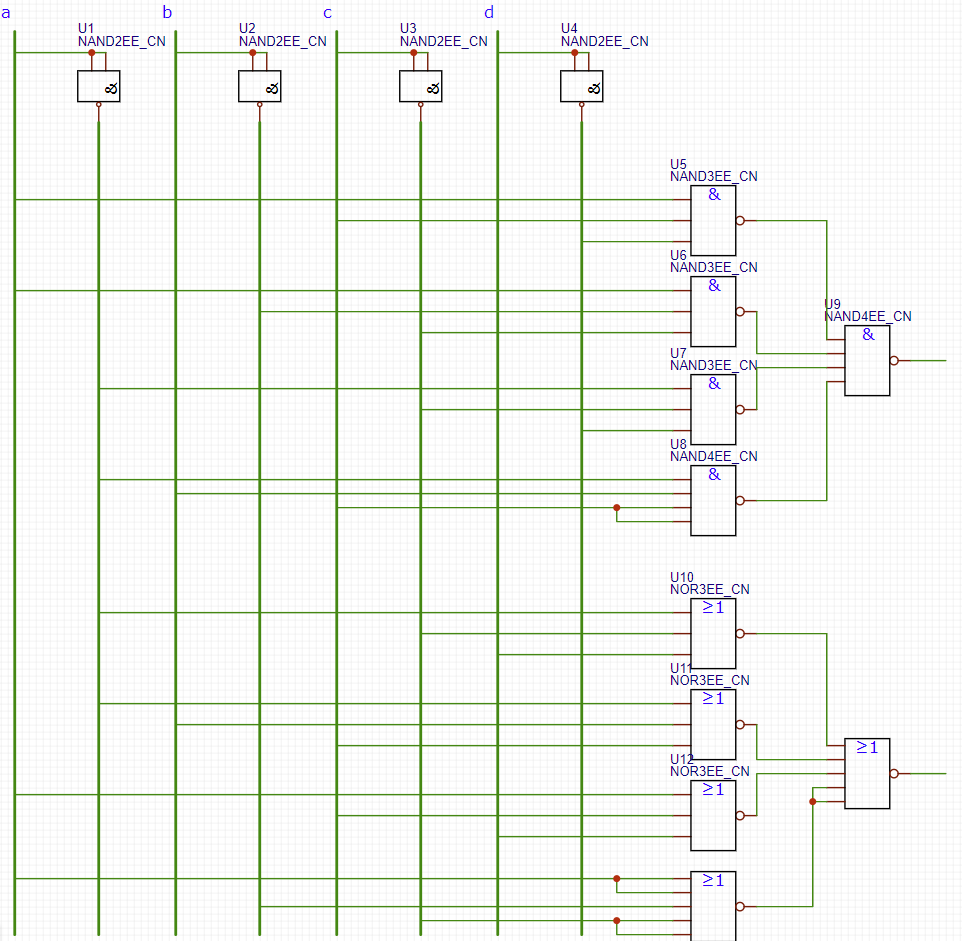
\includegraphics[width=6in]{1.png}
\caption{Schaltbild der NAND-NAND- und NOR-NOR-Realisierung}

\end{figure}

\begin{lstlisting}
library ieee; 
use ieee.std_logic_1164.all; 
use work.pack_2.all;  

entity uut is 
    port (EE_X : in X01_vector(20 downto 13); 
        EE_Y : out X01_vector(20 downto 13)); 
end uut;

architecture structure of uut is

    alias a : x01 is EE_X(20); 
    alias b : x01 is EE_X(19); 
    alias c : x01 is EE_X(18); 
    alias d : x01 is EE_X(17);

    component sn7400 -- 2NAND 
        port (x : in X01_vector (1 to 2); y : out X01); 
    end component;
    component sn7427 -- 3NOR 
        port (x : in X01_vector (1 to 3); y : out X01);
    end component;
    component sn74260 -- 5NOR 
        port (x : in X01_vector (1 to 5); y : out X01); 
    end component;
    component sn7410 -- 3NAND 
        port (x : in X01_vector (1 to 3); y : out X01); 
    end component;
    component sn7420 -- 4NAND 
        port (x : in X01_vector (1 to 4); y : out X01); 
    end component;
signal not_a, not_b, not_c, not_d :X01; 
signal nand_out :X01_vector (1 to 4); 
signal nor_out :X01_vector (1 to 4);

begin 
    -- BLOCK 1 NEGATION
    NA:   sn7400   port map (x(1)=>a,x(2)=>a,y=>not_a); 
    NB:   sn7400   port map (x(1)=>b,x(2)=>b,y=>not_b); 
    NC:   sn7400   port map (x(1)=>c,x(2)=>c,y=>not_c); 
    ND:   sn7400   port map (x(1)=>d,x(2)=>d,y=>not_d);

    -- BLOCK 2 NOR/NOR
    NOR_1:   sn7427   port map 
        (x(1)=>not_a,x(2)=>not_c,x(3)=>d,y=>nor_out(1)); 
    NOR_2:   sn7427   port map 
        (x(1)=>not_a,x(2)=>b,x(3)=>c,y=>nor_out(2)); 
    NOR_3:   sn7427   port map 
        (x(1)=>a,x(2)=>c,x(3)=>d,y=>nor_out(3)); 
    NOR_4:   sn74260   port map 
        (x(1)=>a,x(2)=>not_b,x(3)=>not_c,x(4)=>a,x(5)=>not_c,y=>nor_out(4));
    NOR_RESULT:   sn74260   port map 
        (x(1 to 4)=>nor_out ,x(5)=>nor_out(4),y=>EE_Y(20));
-- BLOCK 3 NAND/NAND
    NAND_1:   sn7410   port map 
        (x(1)=>a,x(2)=>not_c,x(3)=>not_d,y=>nand_out(1));
    NAND_2:   sn7410   port map 
        (x(1)=>a,x(2)=>not_b,x(3)=>not_c,y=>nand_out(2)); 
    NAND_3:   sn7410   port map 
        (x(1)=>not_a,x(2)=>not_c,x(3)=>not_d,y=>nand_out(3)); 
    NAND_4:   sn7420   port map 
        (x(1)=>not_a,x(2)=>b,x(3)=>c,x(4)=>c,y=>nand_out(4));
    NAND_RESULT:   sn7420   port map 
        (x=>nand_out ,y=>EE_Y(19));
end structure;


\end{lstlisting}

\section{Aufgabe 2}

\textbf{binäre Stimulusfolge}
\begin{lstlisting}
stimmap dbb2_08 0000----|11-----
stimmap dbb2_08 0001----|00-----
stimmap dbb2_08 0010----|00-----
stimmap dbb2_08 0011----|00-----
stimmap dbb2_08 0100----|11-----
stimmap dbb2_08 0101----|00-----
stimmap dbb2_08 0110----|11-----
stimmap dbb2_08 0111----|11-----
stimmap dbb2_08 1000----|11-----
stimmap dbb2_08 1001----|11-----
stimmap dbb2_08 1010----|11-----
stimmap dbb2_08 1011----|00-----
stimmap dbb2_08 1100----|00-----
stimmap dbb2_08 1101----|00-----
stimmap dbb2_08 1110----|11-----
stimmap dbb2_08 1111----|00-----
\end{lstlisting}

\textbf{ternäre Stimulusfolge:} 
\begin{lstlisting}
stimmap dbb2_08 0000----|11------
stimmap dbb2_08 000X----|--------
stimmap dbb2_08 0001----|00------
stimmap dbb2_08 00X1----|--------
stimmap dbb2_08 0011----|00------
stimmap dbb2_08 001X----|--------
stimmap dbb2_08 0010----|00------
stimmap dbb2_08 0X10----|--------
stimmap dbb2_08 0110----|11------
stimmap dbb2_08 011X----|--------
stimmap dbb2_08 0111----|11------
stimmap dbb2_08 01X1----|--------
stimmap dbb2_08 0101----|00------
stimmap dbb2_08 010X----|--------
stimmap dbb2_08 0100----|11------
stimmap dbb2_08 X100----|--------
stimmap dbb2_08 1100----|00------
stimmap dbb2_08 110X----|--------
stimmap dbb2_08 1101----|00------
stimmap dbb2_08 11X1----|--------
stimmap dbb2_08 1111----|00------
stimmap dbb2_08 111X----|--------
stimmap dbb2_08 1110----|11------
stimmap dbb2_08 1X10----|--------
stimmap dbb2_08 1010----|11------
stimmap dbb2_08 101X----|--------
stimmap dbb2_08 1011----|00------
stimmap dbb2_08 10X1----|--------
stimmap dbb2_08 1001----|11------
stimmap dbb2_08 100X----|--------
stimmap dbb2_08 1000----|11------
\end{lstlisting}

\section{Aufgabe 3}


\textbf{binäre Stimulation}
\begin{lstlisting}
1 0000---- -> XXXXXXXX                                         
    11----- 
    ^^     ^
2 0001---- -> XXXXXXXX                                         
    00----- 
    ^^     ^
3 0010---- -> XXXXXXXX                                         
    00----- 
    ^^     ^
4 0011---- -> XXXXXXXX                                         
    00----- 
    ^^     ^
5 0100---- -> XXXXXXXX                                         
    11----- 
    ^^     ^
6 0101---- -> XXXXXXXX                                         
    00----- 
    ^^     ^
7 0110---- -> XXXXXXXX                                         
    11----- 
    ^^     ^
8 0111---- -> XXXXXXXX                                         
    11----- 
    ^^     ^
9 1000---- -> XXXXXXXX                                         
    11----- 
    ^^     ^
10 1001---- -> XXXXXXXX                                         
    11----- 
    ^^     ^
11 1010---- -> XXXXXXXX                                         
    11----- 
    ^^     ^
12 1011---- -> XXXXXXXX                                         
    00----- 
    ^^     ^
13 1100---- -> XXXXXXXX                                         
    00----- 
    ^^     ^
14 1101---- -> XXXXXXXX                                         
    00----- 
    ^^     ^
15 1110---- -> XXXXXXXX                                         
    11----- 
    ^^     ^
16 1111---- -> XXXXXXXX                                         
    00----- 
    ^^     ^

\end{lstlisting}

\textbf{ternäre Stimulation}
\begin{lstlisting}
1 0000---- -> XXXXXXXX                                         
    11------
    ^^      
2 000X---- -> XXXXXXXX                                         
    --------
            
3 0001---- -> XXXXXXXX                                         
    00------
    ^^      
4 00X1---- -> XXXXXXXX                                         
    --------
            
5 0011---- -> XXXXXXXX                                         
    00------
    ^^      
6 001X---- -> XXXXXXXX                                         
    --------
            
7 0010---- -> XXXXXXXX                                         
    00------
    ^^      
8 0X10---- -> XXXXXXXX                                         
    --------
            
9 0110---- -> XXXXXXXX                                         
    11------
    ^^      
10 011X---- -> XXXXXXXX                                         
    --------
            
11 0111---- -> XXXXXXXX                                         
    11------
    ^^      
12 01X1---- -> XXXXXXXX                                         
    --------
            
13 0101---- -> XXXXXXXX                                         
    00------
    ^^      
14 010X---- -> XXXXXXXX                                         
    --------
            
15 0100---- -> XXXXXXXX                                         
    11------
    ^^      
16 X100---- -> XXXXXXXX                                         
    --------
            
17 1100---- -> XXXXXXXX                                         
    00------
    ^^      
18 110X---- -> XXXXXXXX                                         
    --------
            
19 1101---- -> XXXXXXXX                                         
    00------
    ^^      
20 11X1---- -> XXXXXXXX                                         
    --------
            
21 1111---- -> XXXXXXXX                                         
    00------
    ^^      
22 111X---- -> XXXXXXXX                                         
    --------
            
23 1110---- -> XXXXXXXX                                         
    11------
    ^^      
24 1X10---- -> XXXXXXXX                                         
    --------
            
25 1010---- -> XXXXXXXX                                         
    11------
    ^^      
26 101X---- -> XXXXXXXX                                         
    --------
            
27 1011---- -> XXXXXXXX                                         
    00------
    ^^      
28 10X1---- -> XXXXXXXX                                         
    --------
            
29 1001---- -> XXXXXXXX                                         
    11------
    ^^      
30 100X---- -> XXXXXXXX                                         
    --------
            
31 1000---- -> XXXXXXXX                                         
    11------
    ^^      

\end{lstlisting}

\end{document}